\documentclass[12pt, a4paper] {ncc}
\usepackage[utf8] {inputenc}
\usepackage[T2A]{fontenc}
\usepackage[english, russian] {babel}
\usepackage[usenames,dvipsnames]{xcolor}
\usepackage{listings,a4wide,longtable,amsmath,amsfonts,graphicx}
\usepackage{indentfirst}
\usepackage{bytefield}
\usepackage{multirow}
\usepackage{float}
\usepackage{caption}
\usepackage{subcaption}
\captionsetup{compatibility=false}
\usepackage{tabularx}

\usepackage[left=2cm,right=2cm,top=2cm,bottom=2cm,bindingoffset=0cm]{geometry}

\begin{document}
\setcounter{figure}{0}
\frenchspacing
\pagestyle{empty}
\begin{center}
                            Университет ИТМО    \\
                        Кафедра систем управления и информатики

\vspace{\stretch{2}}

\end{center}
\vspace{\stretch{2}}
\begin{center}
			Лабораторная работа № 1\\
			по дисциплине: \\
		<<Основы теории автоматического управления>> \\
			Вариант: 5
\end{center}
\vspace{\stretch{3}}
\begin{flushright}
                                    Студент:\\
                                    {\it Куклина М.Д., P3401}\\
                                    Преподаватель: \\
                                    {\it Кремлев А.С.}
\end{flushright}
\vspace{\stretch{4}}
\begin{center}
                             Санкт-Петербург, 2018
\end{center}
\newpage

\section{Математические модели динамических систем и соответствующие им схемы моделирования}

	См. рисунки 1-4.

		\begin{figure}[ht!]
    		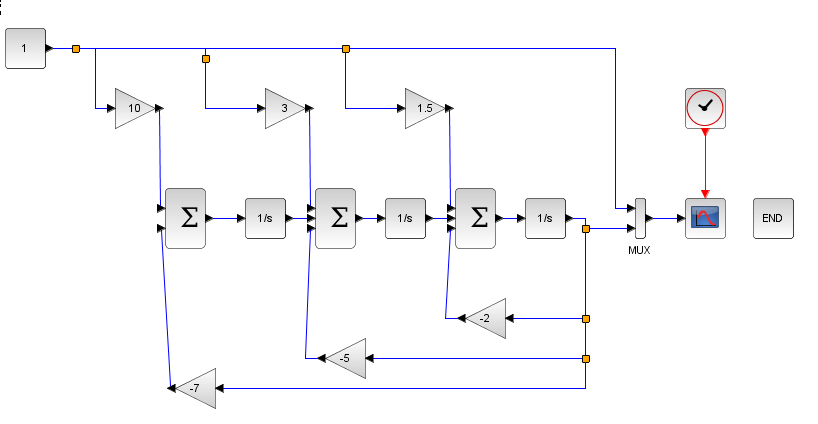
\includegraphics[scale=0.5]{./modelio1t.png}
			\caption{Схема моделирования для входного воздействия $u = 1(t)$ для модели вход-выход}
		\end{figure}

		\begin{figure}[ht!]
    		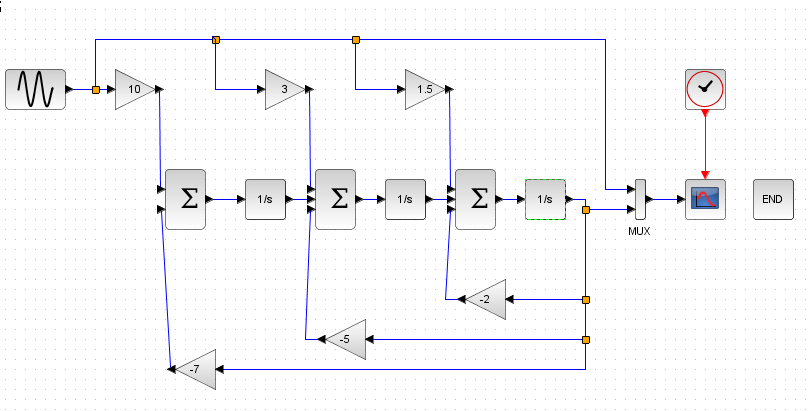
\includegraphics[scale=0.5]{./modeliosin.png}
			\caption{Схема моделирования для входного воздействия $u = 2\sin(t)$ для модели вход-выход}
		\end{figure}

		\begin{figure}[ht]
    		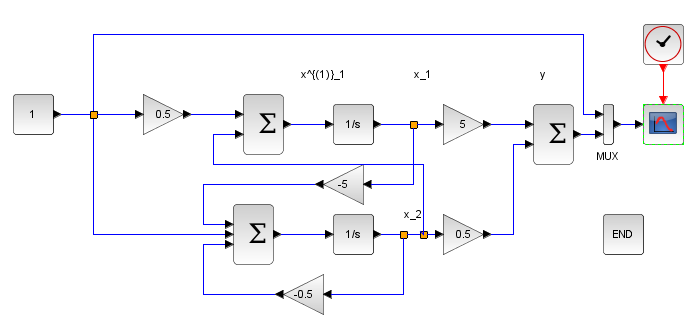
\includegraphics[scale=0.5]{./modelios1t.png}
			\caption{Схема моделирования для входного воздействия $u = 1(t)$ для модели вход-состояние-выход}
		\end{figure}

		\begin{figure}[ht]
    		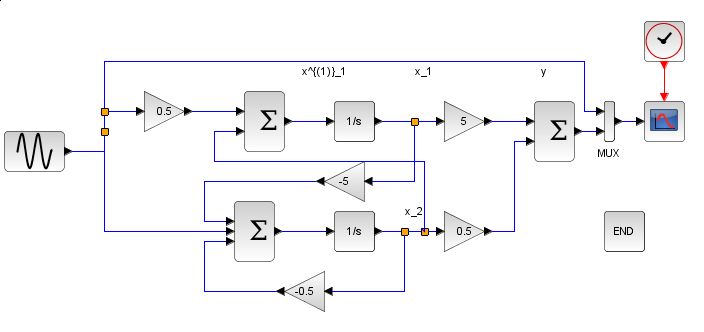
\includegraphics[scale=0.5]{./modeliossin.png}
			\caption{Схема моделирования для входного воздействия $u = 2\sin(t)$ для модели вход-состояние-выход}
		\end{figure}


\section{Расчёт начальных условий интеграторов}

		Дифференциальное уравнение.\\
		$y^{(3)} + 2 y^{(2)} + 5 y^{(1)} + 7 y = 1.5 u^{(2)} + 3 u^{(1)} + 10 u $ \\
		$s = \frac{d} {d t}$ \\
		$s^3y + 2 s^2 y  + 5 s y + 7 y = 1.5 s^2 u + 3s u + 10 u$\\
		$y = \frac{1}{s} (1.5 u - 2 y ) + \frac{1}{s^2} (3 u - 5 y) + \frac{1}{s^3}(10 u - 7 y)$
		\begin{enumerate}
			\item Вычисление начального условия первого интегратора. \\
				  $z_1 = y \to z_1(0) = y(0) = 1 $
			\item Вычисление начального условия второго интегратора. \\
				  $\dot{z_1} = \dot{y} = z_2 + b_2 u - a_2 y$ \\
				  $z_2 = \dot{y} - b_2  u + a_2 y $ \\
				  $z_2(0) = \dot{y}(0) - b_2  u(0) + a_2 y(0) $ \\
				  $z_2(0) = -0.5 - 1.5 \times 0 + 2 \times 1$ \\
				  $z_2(0) = 1.5$
			\item Вычисление начального условия третьего интегратора. \\
				  $\dot{z_2} = z_3 + b_1 u - a_1 y $ \\
				  $z_3 = \dot{z_2} - b_1 u + a_1 y $ \\
				  $z_3 = \ddot{y} - b_2 \dot{u} + a_2 \dot{y} - b_1 u + a_1 y$ \\
				  $z_3(0) = 0 - 1.5 \times 0 + 2 \times (-0.5) - 3 \times 0 + 5 \times 1$ \\
				  $z_3(0) = -1 + 5 = 4$
		\end{enumerate}

	\section{Результаты моделрования}
		См. рисунки 5-10.

		\begin{figure}[ht!]
    		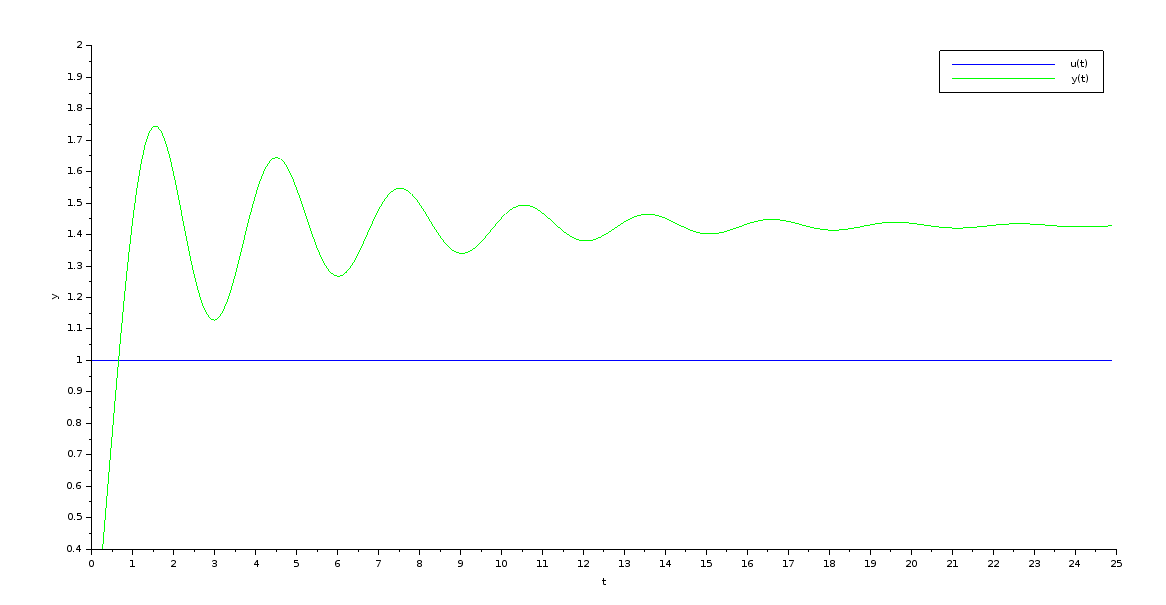
\includegraphics[scale=0.4]{./plotio1t1.png}
			\caption{График при входном воздействии $u = 1(t)$ для модели вход-выход}
		\end{figure}

		\begin{figure}[ht!]
    		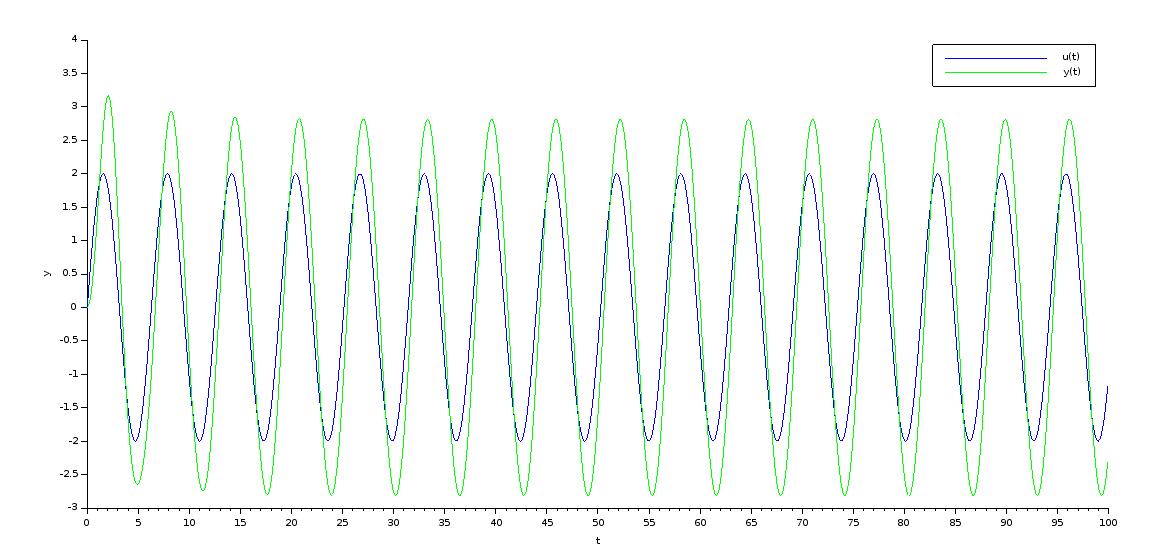
\includegraphics[scale=0.4]{./plotiosin.png}
			\caption{График при входном воздействии $u = 2\sin(t)$ для модели вход-выход}
		\end{figure}

		\begin{figure}[ht!]
    		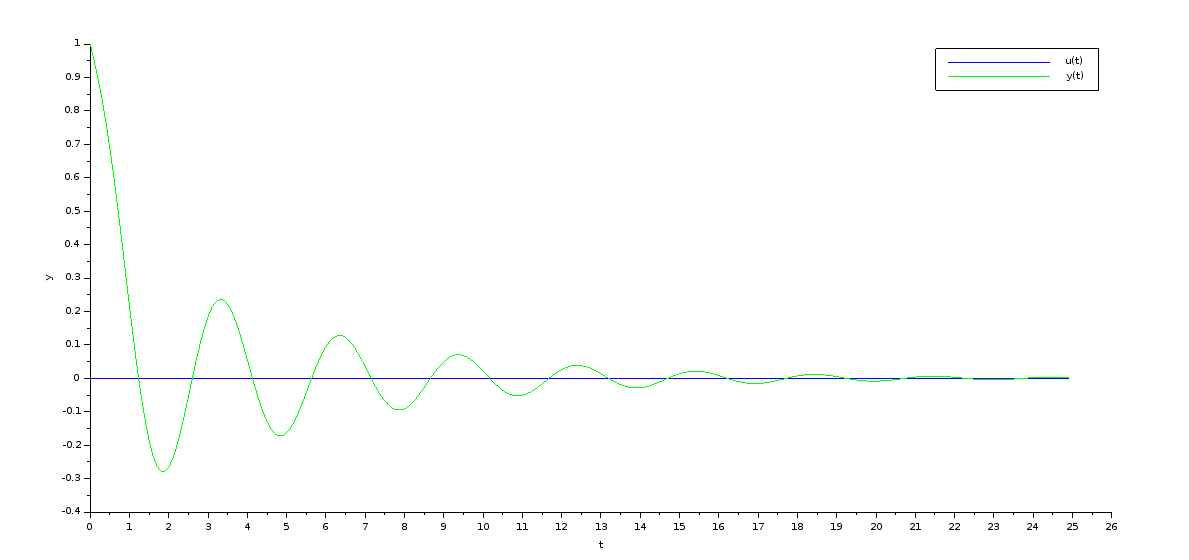
\includegraphics[scale=0.4]{./plotiofree.png}
			\caption{График при нулевом входном воздействии и с ненулевыми начальными условиями для модели вход-выход}
		\end{figure}

		\begin{figure}[ht]
    		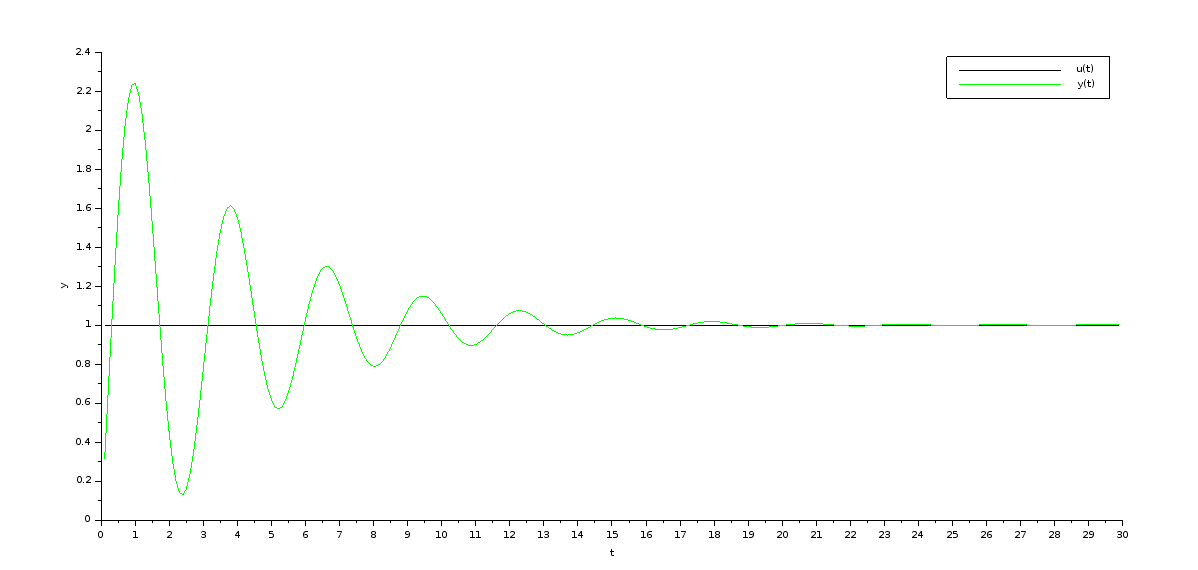
\includegraphics[scale=0.4]{./plotios1t.png}
			\caption{График при входном воздействии $u = 1(t)$ для модели вход-состояние-выход}
		\end{figure}

		\begin{figure}[ht]
    		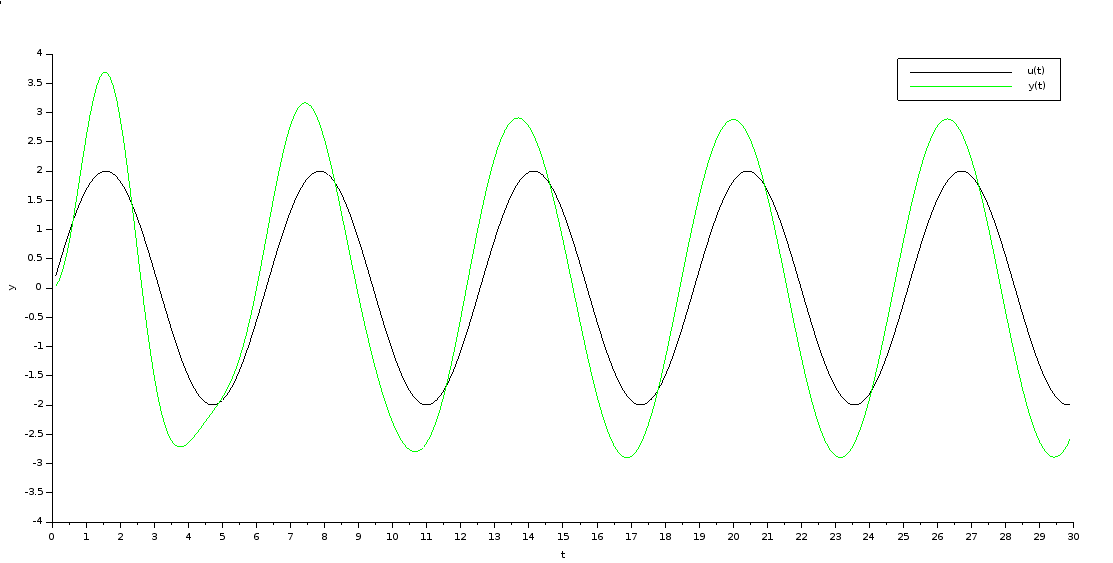
\includegraphics[scale=0.4]{./plotiossin.png}
			\caption{График при входном воздействии $u = 2\sin(t)$ для модели вход-состояние-выход}
		\end{figure}

		\begin{figure}[ht]
    		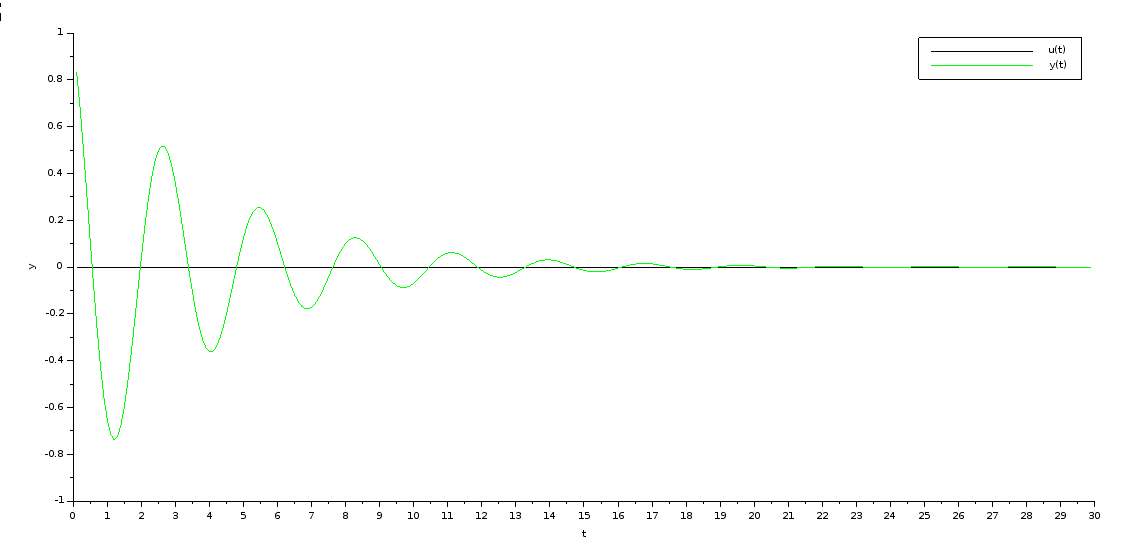
\includegraphics[scale=0.4]{./plotiosfree.png}
			\caption{График при нулевом входном воздействии и с ненулевыми начальными условиями для модели вход-состояние-выход}
		\end{figure}


    \section{Вывод}

        В ходе выполнения лабораторной работы происходили исследования моделей вход-выход и вход-состояние-выход в
        системе Scilab/Xcos. В результате выяснилось, что возможности Xcos в рамаках данной лабораторной работы
        полностью соответствуют возможностям SIMULINK.


\end{document}
